\documentclass[twocolumn]{ctexart}
\usepackage{amsmath}
\usepackage{tikz}
\newcommand{\sol}[1]{\subsection*{#1}\noindent\textbf{解:}

}
\begin{document}
	\sol{2-4}
	从$O$点垂直$\vec{\omega}$向外建立极轴,取随绳转动的参考系. 记绳的线密度为$\eta=m/L$.
	
	在转动参考系中,绳子保持静止,所受惯性离心力
	\begin{align*}
		F_r=\int_{x}^{L}{\omega}^2r\eta\mathrm{d}r
		&=\frac{{\omega}^2\eta\left(L^2-x^2\right)}{2}\\
		&=\frac{m\omega^2\left(L^2-x^2\right)}{2L}.
	\end{align*}
	
	设内侧绳子拉力为$T$,由非惯性系中的牛顿第二定律有
	$$F_T(x)=F_r=\frac{m\omega^2\left(L^2-x^2\right)}{2L}.$$
	
	\sol{2-6}
	\subsubsection*{(1)}
	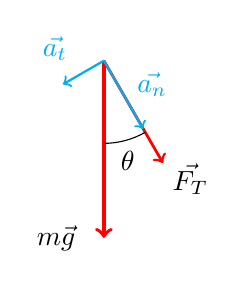
\begin{tikzpicture}[scale=1.5]
		%力
		\draw[line width=1.3pt, color=red][->] (0, 0)--(0,-1.5);
		\draw[line width=1pt, color=red][->] (0, 0)--(0.5, -1.732/2);
		\draw(0, -0.7) arc (270:300:0.7);
		\node[right] at(-0.65, -1.5) {$m\vec{g}$};
		\node[right] at(0.5, -1) {$\vec{F_T}$};
		\node[right] at(0.06, -0.85) {$\theta$};
		%加速度
		\draw[line width=0.8pt, color=cyan][->] (0, 0)--(1/3, -1.732/3);
		\draw[line width=0.8pt, color=cyan][->] (0, 0)--(-1.732/5, -1/5);
		\node[right, color=cyan] at(0.2, -0.2) {$\vec{a_n}$};
		\node[right, color=cyan] at(-0.6, 0.1) {$\vec{a_t}$};
	\end{tikzpicture}
	
	受力分析及加速度正交分解的图示如上.
	
	运动学定律
	\begin{align}
		a_n=\frac{v^2}{R}
	\end{align}
	
	牛顿第二定律
	\begin{align}
		&F_T+mg\cos\theta=ma_n\\
		&mg\sin\theta=ma_t
	\end{align}
	
	由(1)(2)(3)解得$\vec{F_T}$和$\vec{a_t}$的大小
	\begin{align*}
		&F_T=m\left(\frac{v^2}{R}-g\cos\theta\right),\\
		&a_t=g\sin\theta.
	\end{align*}
	
	$\vec{F_T}$的方向沿绳指向圆心,当$a_t>0$时,$\vec{a_t}$的方向与物体速度方向相同,$a_t<0$则相反.
	
	\subsubsection*{(2)}
	由受力分析易得$\vec{a_t}$的方向与重力和物体运动方向的夹角有关. 当$0<\theta<180^\circ{}$时,$\vec{a_t}$的方向与运动方向相同,当$180^\circ{}<\theta<360 ^\circ{}$(物体在右半侧)时,$\vec{a_t}$的方向与运动方向相反,其余情况$\vec{a_t}$大小为$0$.
	
	\sol{2-8}
	\subsubsection*{(1)}
	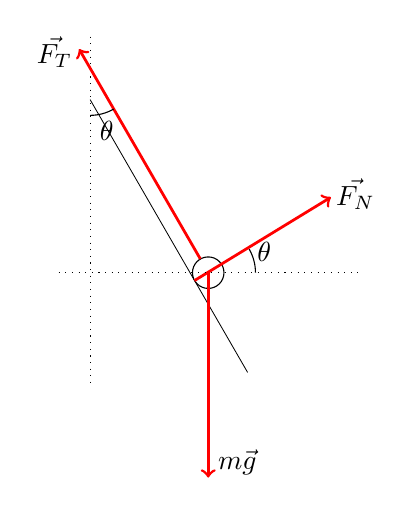
\begin{tikzpicture}[scale=2]
		\draw[dotted] (0, 0.2)--(0,-2);
		\draw[line width=0.3pt] (0, 0)--(1*0.7, -1.732*0.7);
		\draw(0.75, -1.299) circle (0.1);
		\draw[line width=0.3pt] (0,-0.2)--(1, -1.932);
		\draw[line width=1pt,color=red][->] (0.663,-1.349)--(1.529,-0.82);
		\draw[dotted] (-0.2, -1.299)--(1.7,-1.299);
		\draw[line width=1pt,color=red][->] (0.75, -1.299)--(0.75, -2.6);
		\draw[line width=1pt,color=red][->] (0.7, -1.212)--(-0.07, 0.121);
		\draw(0,-0.3) arc(270:300:0.3);
		\draw(1.05, -1.299) arc(0:30:0.3);
		\node[right] at(-0.4, 0.1) {$\vec{F_T}$};
		\node[right] at(1.5, -0.8) {$\vec{F_N}$};
		\node[right] at(0.75, -2.5) {$m\vec{g}$};
		\node[right] at(0, -0.4) {$\theta$};
		\node[right] at(1, -1.17) {$\theta$};
	\end{tikzpicture}

	小球的加速度大小
	\setcounter{equation}{0}
	\begin{align}
		a=m\omega^2l\sin\theta
	\end{align}
	
	牛顿第二定律
	
	\begin{align}
		&F_T-mg\cos\theta=a\sin\theta\\
		&F_N-mg\sin\theta=-a\cos\theta
	\end{align}
	由(1)(2)(3)解得
	\begin{align}
		&F_T=m\left(g\cos\theta+\omega^2l\sin^2\theta\right)\\
		&F_N=m\left(g\sin\theta-\omega^2l\sin\theta\cos\theta\right)
	\end{align}
	\subsubsection*{(2)}
	当小球恰好要离开锥面时,有$F_N=0$.
	
	在(5)中令$F_N=0$,得
	$$\omega_0=\sqrt{\frac{g}{l\cos\theta}}.$$
	
	代入(4)式得
	$$F_T=\frac{mg}{\cos\theta}.$$
	\sol{2-10}
	\noindent
	\textbf{注:此题有两个版本,分别位于2015年第一次印刷(旧版)及2018年第四次印刷(新版)的大学物理课本. 具体区别为方形物体的高度$h_0$是否被标注,即是否忽略方形物体的高度. 由于我使用的是旧版电子课本,我将把两个版本的题解分开列在下方.}
	
	\noindent
	\textbf{旧版($h_0$不作标注):}
	
	设全过程中滑轮左侧绳长的减少量为$\Delta x$,由几何关系得
	$$\Delta x=\frac{h}{\sin30^\circ{}}-\frac{h}{\sin60^\circ{}}=\left(4-\frac{4\sqrt{3}}{3}\right)\mathrm{m}.$$
	
	力$F$作正功
	$$W=F\cdot\Delta x=\left(48-16\sqrt{3}\right)\mathrm{J}=20.287\ \mathrm{J}.$$
	
	\noindent
	\textbf{新版($h_0$作标注):}
	
	设全过程中滑轮左侧绳长的减少量为$\Delta x$,由几何关系得
	$$\Delta x=\frac{h-h_0}{\sin30^\circ{}}-\frac{h-h_0}{\sin60^\circ{}}=1.2\left(2-\frac{2\sqrt{3}}{3}\right)\ \mathrm{m}.$$
	
	力$F$作正功
	$$W=F\cdot\Delta x=14.4\left(2-\frac{2\sqrt{3}}{3}\right)\ \mathrm{J}=12.172\ \mathrm{J}.$$
	
	\sol{2-13}
	质点的速度
	\begin{align*}
		\vec{v}&=\frac{\mathrm{d}\vec{x}}{\mathrm{d}t}\\
		&=\left(5\hat{\mathbf{i}}+t\hat{\mathbf{j}}\right)\ \mathrm{m\cdot s^{-1}}
	\end{align*}
	
	加速度
	\begin{align*}
		\vec{a}&=\frac{\mathrm{d}\vec{v}}{\mathrm{d}t}\\
		&=t\hat{\mathbf{j}}\ \mathrm{m\cdot s^{-2}}
	\end{align*}

	牛顿第二定律
	
	$$\vec{F}=m\vec{a}=0.5\hat{\mathbf{j}}\ \mathrm{N}$$
	
	外力对质点做功
	\begin{align*}
		A&=\int_{t=2\ \mathrm{s}}^{t=4\ \mathrm{s}}\vec{F}\cdot\mathrm{d}\vec{r}\\
		&=\int_{2}^{4 }0.5\hat{\mathbf{j}}\cdot\left(5\hat{\mathbf{i}}+t\hat{\mathbf{j}}\right)\mathrm{d}t\ \mathrm{J}\\
		&=\int_{2}^{4}0.5t\mathrm{d}t\ \mathrm{J}\\
		&=3\ \mathrm{J}
	\end{align*}
	
	\sol{2-14}
	%记两颗中子星分别对应下标1和2. 列出两颗星的牛顿第二定律方程
	%\setcounter{equation}{0}
	%\begin{align}
		%&m_1\frac{\mathrm{d}^2\mathbf{r}_1}{\mathrm{d}t^2}=\frac{Gm_1m_2}{r_{12}^2}\hat{\mathbf{r}_{12}}\\
	%	%&m_2\frac{\mathrm{d}^2\mathbf{r}_2}{\mathrm{d}t^2}=\frac{Gm_1m_2}{r_{12}^2}\hat{\mathbf{r}_{21}}
	%\end{align}
	
	%我们有$\hat{\mathbf{r}_{12}}=-\hat{\mathbf{r}_{21}}$,将(1)(2)两式左侧的质量消去后,用(2)减去(1)得
	%\begin{align}
	%	\frac{\mathrm{d}^2\mathbf{r}}{\mathrm{d}t^2}=-\frac{G\left(m_1+m_2\right)}{r^2}\hat{\mathbf{r}}
	%\end{align}
	
	%其中$\mathbf{r}=\mathbf{r}_2-\mathbf{r}_1$. 因为由方程(3)以及一定的初始条件可以完全确定中子星2相对中子星1的运动状态,所以从运动学角度上,我们可以认为,中子星2相对1的运动可以等效于一个质量为$m$(这质量终将消去,所以其实际值并不重要)的质点相对于一个质量为$\left(m_1+m_2\right)\gg m$的质点(忽略这个质点的运动)的运动.
	
	由对称性得两颗中子星的速度等大反向,设中子星质量为$m$,速率为$v$,相互距离为$r$,初始距离为$r_0$. 引力势能
	\setcounter{equation}{0}
	$$E_g=-\frac{Gm^2}{r}.$$

	由能量守恒
	$$-\frac{Gm^2}{r_0}=-\frac{Gm^2}{r_0/2}+\frac{1}{2}mv^2+\frac{1}{2}mv^2$$
	
	解得
	$$v=\sqrt{\frac{Gm}{r_0}}.$$
	
	代入数值得
	$$v=8.17\times 10^4\ \mathrm{m/s}.$$
	\sol{2-15}
	设弹簧伸长量为$x$,机械能守恒
	\setcounter{equation}{0}
	\begin{align}\frac{1}{2}mv_0^2=\frac{1}{2}m\left(\frac{v_0}{2}\right)^2+\frac{1}{2}kx^2\end{align}
	
	胡克定律
	\begin{align}F=kx\end{align}
	
	由(1)(2)解得
	$$F=\frac{v_0}{2}\sqrt{3km}.$$
	\sol{2-16}
	设摩擦力做功$W_f$,由能量守恒
	$$mgR+W_f=\frac{1}{2}mv^2$$
	解得
	$$W_f=\frac{1}{2}mv^2-mgR.$$
	
	代入数值得
	$$W_f=-42.4\ \mathrm{J}.$$
	\sol{2-17}
	牛顿第二定律
	$$F-kx-\mu mg=m\frac{\mathrm{d}^2x}{\mathrm{d}t^2}$$
	
	整理得
	$$\frac{\mathrm{d}^2}{\mathrm{d}t^2}\left(x+\frac{\mu mg-F}{k}\right)=-\frac{k}{m}\left(x+\frac{\mu mg-F}{k}\right).$$
	
	可以判断物体在第一次到达最右端之前做简谐运动,劲度系数为$k/m$,等效原点为$x_0=(F-\mu mg)/k$. 物体由静止开始运动,因此振幅$A_0=x$. 物体运动的最远点坐标为$x_1=2(F-\mu mg)/k$.
	
	由于力$F$可以认为是保守的,由于摩擦力的耗散作用,整个系统在运动过程中机械能(含力$F$的势能)会不断减少,因此可以确定第一次达到的最右侧点就是最远位置. 弹性势能
	$$E_s=\frac{1}{2}kx_1^2=\frac{2}{k}\left(F-\mu mg\right)^2.$$
	\sol{2-20}
	\noindent
	动量定理:
	
	\begin{align*}
		&\vec{v_1}=\omega R\hat{\mathbf{j}}\\
		&\vec{v_2}=-\omega R\hat{\mathbf{i}}
	\end{align*}

	动量定理
	\begin{align*}
		\vec{I}&=m\left(\vec{v_2}-\vec{v_1}\right)\\
		&=-m\omega R\hat{\mathbf{i}}-m\omega R\hat{\mathbf{j}}
	\end{align*}

	\noindent
	积分法:
	
	物体做匀速圆周运动,合力指向圆心,满足
	$$\vec{F}=-m\omega^2R\cos(\omega t)\hat{\mathbf{i}}-m\omega^2R\sin(\omega t)\hat{\mathbf{j}}.$$
	
	冲量
	\begin{align*}
		\vec{I}&=\int_{0}^{\frac{\pi}{2\omega}}\vec{F}\mathrm{d}t\\
		&=\int_{0}^{\frac{\pi}{2\omega}}-m\omega^2R\cos(\omega t)\hat{\mathbf{i}}-m\omega^2R\sin(\omega t)\hat{\mathbf{j}}\mathrm{d}t\\
		&=\left[-m\omega R\sin(\omega t)\hat{\mathbf{i}}+m\omega R\cos(\omega t)\hat{\mathbf{j}}\right]_0^{\frac{\pi}{2\omega}}\\
		&=-m\omega R\hat{\mathbf{i}}-m\omega R\hat{\mathbf{j}}
	\end{align*}

	与用动量定理所得结果相同.
	\sol{2-22}
	动量定理
	\begin{align*}
		&\left(m_1+m_2\right)\left(v_A-0\right)=F\Delta t_1\\
		&m_2\left(v_B-v_A\right)=F\Delta t_2
	\end{align*}
	
	解得
	\begin{align*}
		&v_A=\frac{F\Delta t_1}{m_1+m_2}\\
		&v_B=\frac{F\Delta t_1}{m_1+m_2}+\frac{F\Delta t_2}{m_2}
	\end{align*}
	\sol{2-23}
	在沿绳的自由度上使用牛顿第二定律,
	$$mg=(m+m)a$$
	得$a=g/2$.
	
	记$x_1=0.2\ \mathrm{m}$为BC间绳长. 设经时间$t_1$后C开始运动,由运动学定律,
	$$x_1=\frac{1}{2}at_1^2$$
	
	得$t_1=\sqrt{4x_1/g}$. 代入数值得$t_1=2/7\ \mathrm{s}=0.286\ \mathrm{s}$.
	
	由动量定理,
	$$mgt_1=3mv_C,$$
	
	其中$v_C$为C开始运动的速率. 代入数值解得$v_C=0.933\ \mathrm{m/s}$.
	\sol{2-24}
	三艘船前后依次编号为1,2,3.
	
	在2船参考系中,两个物体同时以速率$u$向前向后抛出,2船速度大小不变.
	
	动量守恒
	\begin{align*}
		&m'v+m(v+u)=\left(m'+m\right)v_1'\\
		&m'v+m(v-u)=\left(m'+m\right)v_3'\\
		&v_2'=v
	\end{align*}

	解得
	\begin{align*}
		&v_1'=v+\frac{mu}{m'+m}\\
		&v_2'=v\\
		&v_3'=v-\frac{mu}{m'+m}
	\end{align*}
	
	\sol{2-28}
	设向下滑的距离为$x$,绳子的线密度为$\eta$.
	
	牛顿第二定律
	\setcounter{equation}{0}
	\begin{align}
		\eta(a+x)g\sin\alpha=\eta La
	\end{align}
	
	又
	\begin{align}
		a=\frac{\mathrm{d}v}{\mathrm{d}t}=\frac{\mathrm{d}v}{\mathrm{d}x}\cdot\frac{\mathrm{d}x}{\mathrm{d}t}=v\frac{\mathrm{d}v}{\mathrm{d}x}
	\end{align}
	由(1)(2)整理得
	$$Lv\mathrm{d}v=(ag\sin\alpha+xg\sin\alpha)\mathrm{d}x$$
	
	积分
	$$\int_{0}^{v}Lv\mathrm{d}v=\int_{0}^{L-a}(ag\sin\alpha+xg\sin\alpha)\mathrm{d}x$$
	
	得
	$$Lv^2=\left(L^2-a^2\right)g\sin\alpha$$
	
	即
	$$v=\sqrt{\frac{\left(L^2-a^2\right)g\sin\alpha}{L}}$$
\end{document}